\begin{columns}
\begin{column}{.79\textwidth}
\begin{longtable}{ m{10cm} m{2cm} m{18cm} m{2cm} m{23cm} }
  \begin{minipage}{8cm}
%#vertical 24
\begin{tikzpicture}[>=latex,line join=bevel,]
%%
\node (ldb) at (100bp,130bp) [draw=black,rectangle] {LDB};
  \node (h_st) at (0bp,10bp) [draw=black,rectangle] {ST};
  \node (add4) at (0bp,34bp) [draw=black,rectangle] {ADD};
  \node (add3) at (52bp,130bp) [draw=black,rectangle] {ADD};
  \node (add2) at (52bp,178bp) [draw=black,rectangle] {ADD};
  \node (add1) at (0bp,202bp) [draw=black,rectangle] {ADD};
  \node (ldi2) at (100bp,226bp) [draw=black,rectangle] {LDI};
  \node (ldi1) at (0bp,226bp) [draw=black,rectangle] {LDI};
  \node (merge) at (52bp,58bp) [draw=black,rectangle] {MERGE};
  \node (split) at (52bp,106bp) [draw=black,rectangle] {SPLIT};
  \coordinate (aux) at (100bp,154bp);
  \node (mul1) at (100bp,202bp) [draw=black,rectangle] {MUL};
  \node (buff) at (52bp,154bp) [draw=black,rectangle] {BUFFER};
\draw [-{Latex[length=5mm]}, thick] (ldi2) -- (add1);
  \draw [->,solid] (add4) -- (h_st);
  \draw [->,solid] (add2) -- (buff);
  \draw [->,solid] (aux) -- (add3);
  \draw [->,solid] (ldb) -- (split);
  \draw [->,solid] (buff) -- (add3);
  \draw [->,solid] (ldb) -- (merge);
  \draw [->,solid] (ldi2) -- (mul1);
  \draw [->,solid] (ldi1) -- (mul1);
  \draw [solid] (add2) -- (aux);
  \draw [->,solid] (merge) -- (add4);
  \draw [->,solid] (mul1) -- (add2);
  \draw [->,solid] (add3) -- (split);
  \draw [->,solid] (split) -- (45bp,82bp) -- (merge);
  \draw [->,solid] (split) -- (59bp,82bp) -- (merge);
  \draw [->,solid] (ldi1) -- (add1);
  \draw [->,solid] (add1) -- (add2);
  \draw [->,solid] (add2) -- (add4);
%
\end{tikzpicture}


  \end{minipage}
&
$\longrightarrow$
&

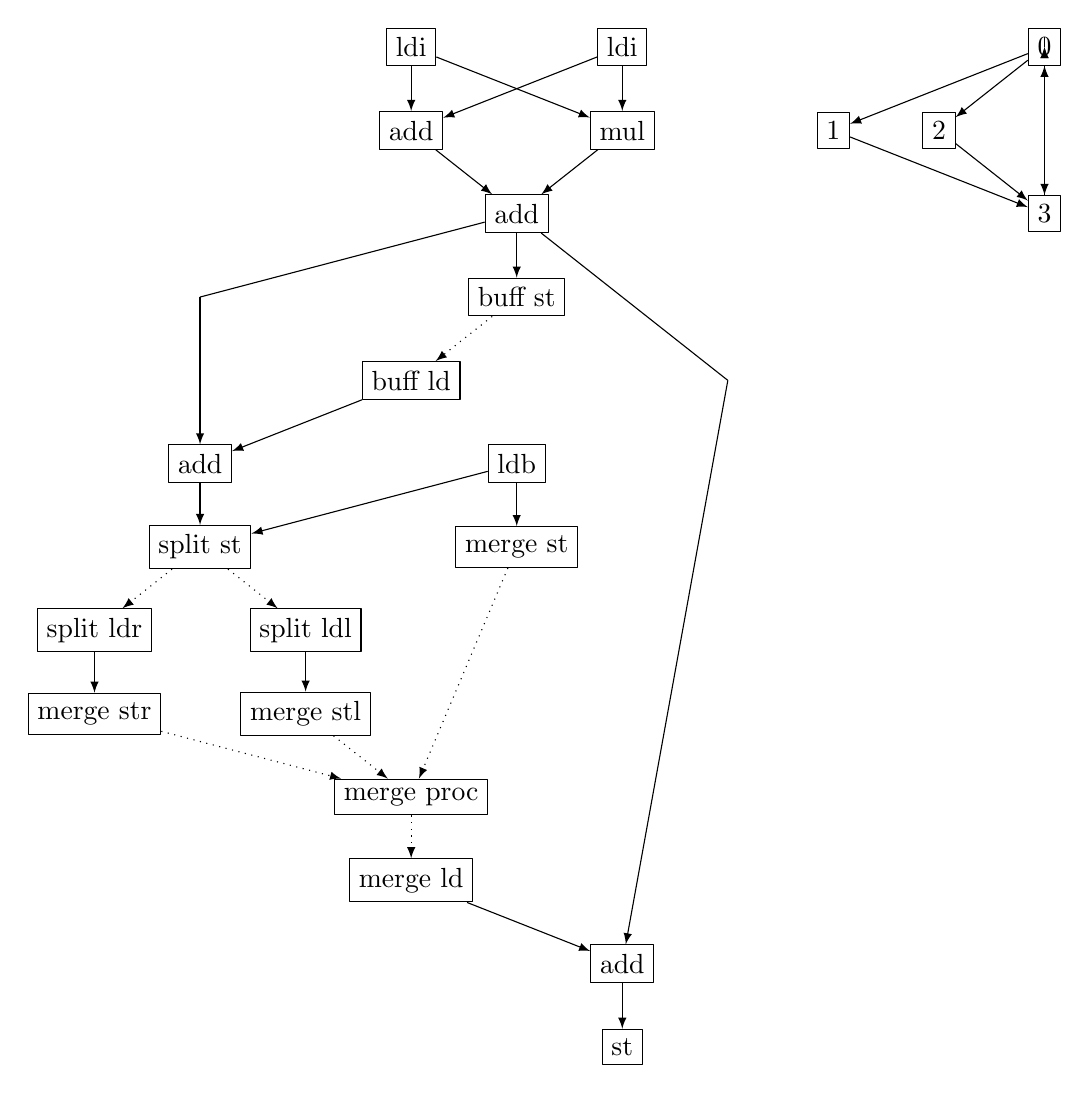
\begin{tikzpicture}[>=latex,line join=bevel,]
%%
\node (ldb) at (152bp,220bp) [draw=black,rectangle] {ldb};
  \node (merge_stl_3) at (76bp,130bp) [draw=black,rectangle] {merge stl};
  \node (mul1) at (190bp,340bp) [draw=black,rectangle] {mul};
  \node (merge_stbuff_3) at (152bp,190bp) [draw=black,rectangle] {merge st};
  \node (split_ldr_2) at (0bp,160bp) [draw=black,rectangle] {split ldr};
  \node (1) at (266bp,340bp) [draw,rectangle] {1};
  \node (0) at (342bp,370bp) [draw,rectangle] {0};
  \node (3) at (342bp,310bp) [draw,rectangle] {3};
  \node (2) at (304bp,340bp) [draw,rectangle] {2};
  \node (buff_st_1) at (152bp,280bp) [draw=black,rectangle] {buff st};
  \node (merge_ld_3) at (114bp,70bp) [draw=black,rectangle] {merge ld};
  \node (split_ldl_2) at (76bp,160bp) [draw=black,rectangle] {split ldl};
  \node (split_st_2) at (38bp,190bp) [draw=black,rectangle] {split st};
  \coordinate (auto_buff_ld_5) at (228bp,250bp);
  \coordinate (auto_buff_ld_4) at (38bp,280bp);
  \node (h_st) at (190bp,10bp) [draw=black,rectangle] {st};
  \node (add4) at (190bp,40bp) [draw=black,rectangle] {add};
  \node (add3) at (38bp,220bp) [draw=black,rectangle] {add};
  \node (add2) at (152bp,310bp) [draw=black,rectangle] {add};
  \node (add1) at (114bp,340bp) [draw=black,rectangle] {add};
  \node (merge_proc_3) at (114bp,100bp) [draw=black,rectangle] {merge proc};
  \node (ldi2) at (190bp,370bp) [draw=black,rectangle] {ldi};
  \node (ldi1) at (114bp,370bp) [draw=black,rectangle] {ldi};
  \node (buff_ld_1) at (114bp,250bp) [draw=black,rectangle] {buff ld};
  \node (merge_str_3) at (0bp,130bp) [draw=black,rectangle] {merge str};
  \draw [->,solid] (add4) -- (h_st);
  \draw [black,->,solid] (0) -- (2);
  \draw [->,solid] (merge_ld_3) -- (add4);
  \draw [->,solid] (ldi1) -- (add1);
  \draw [black,->,solid] (3) -- (0);
  \draw [->,solid] (split_ldr_2) -- (merge_str_3);
  \draw [->,solid] (ldi1) -- (mul1);
  \draw [solid] (add2) -- (auto_buff_ld_5);
  \draw [->,solid] (ldb) -- (merge_stbuff_3);
  \draw [->,solid] (add1) -- (add2);
  \draw [->,solid] (add2) -- (buff_st_1);
  \draw [->,solid] (add3) -- (split_st_2);
  \draw [->,solid] (auto_buff_ld_5) -- (add4);
  \draw [->,dotted] (split_st_2) -- (split_ldr_2);
  \draw [->,solid] (ldb) -- (split_st_2);
  \draw [->,dotted] (merge_str_3) -- (merge_proc_3);
  \draw [black,->,solid] (0) -- (3);
  \draw [->,dotted] (merge_stl_3) -- (merge_proc_3);
  \draw [black,->,solid] (2) -- (3);
  \draw [->,solid] (split_ldl_2) -- (merge_stl_3);
  \draw [->,solid] (ldi2) -- (add1);
  \draw [->,dotted] (split_st_2) -- (split_ldl_2);
  \draw [->,dotted] (merge_stbuff_3) -- (merge_proc_3);
  \draw [->,solid] (mul1) -- (add2);
  \draw [black,->,solid] (0) -- (1);
  \draw [->,solid] (ldi2) -- (mul1);
  \draw [->,dotted] (buff_st_1) -- (buff_ld_1);
  \draw [->,dotted] (merge_proc_3) -- (merge_ld_3);
  \draw [black,->,solid] (0) -- (0);
  \draw [black,->,solid] (0) -- (0);
  \draw [->,solid] (auto_buff_ld_4) -- (add3);
  \draw [solid] (add2) -- (auto_buff_ld_4);
  \draw [->,solid] (buff_ld_1) -- (add3);
  \draw [black,->,solid] (1) -- (3);
%
\end{tikzpicture}


&
$\longrightarrow$
&

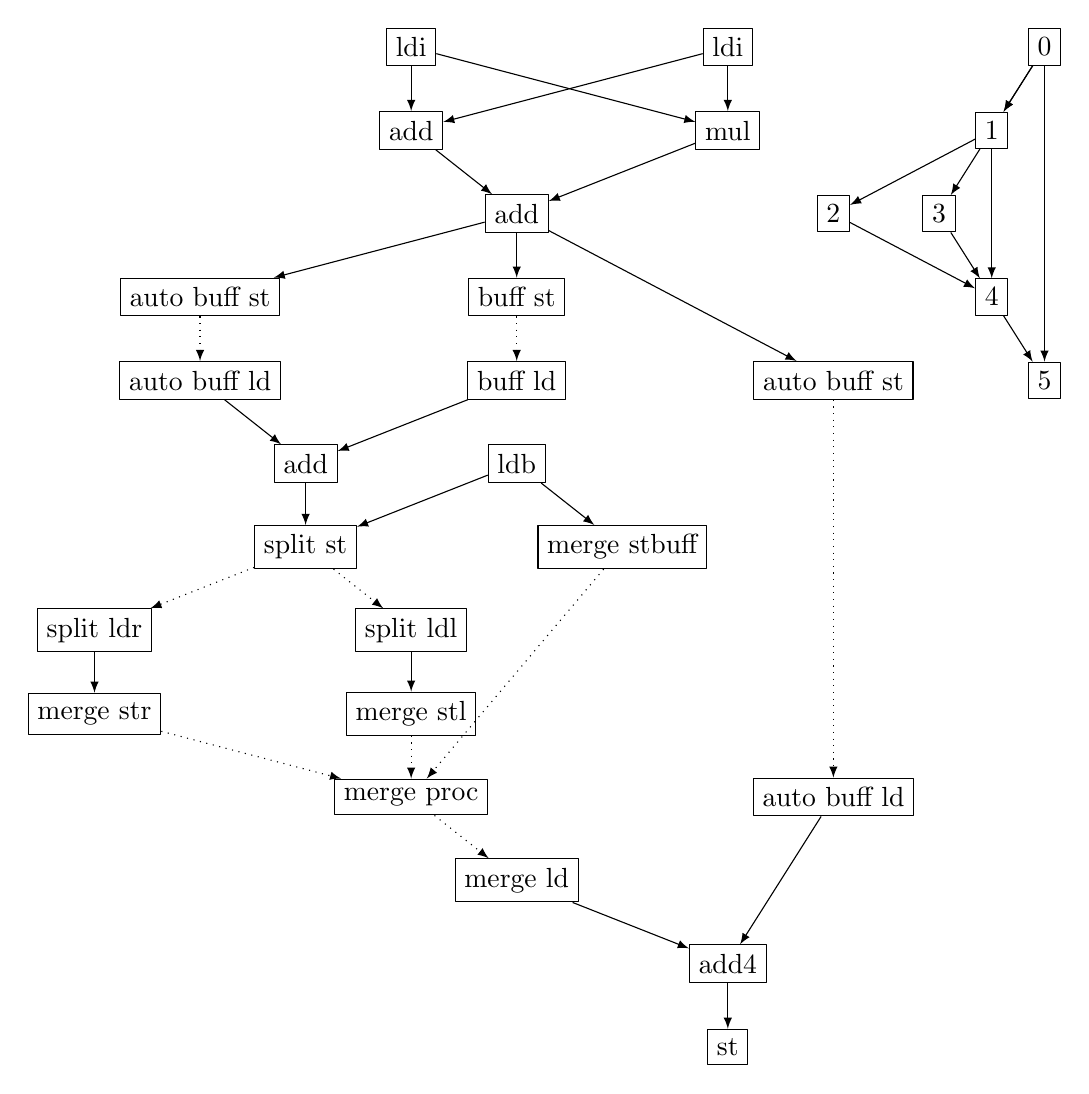
\begin{tikzpicture}[>=latex,line join=bevel,]
%%
\node (ldb) at (152bp,220bp) [draw=black,rectangle] {ldb};
  \node (merge_stl_3) at (114bp,130bp) [draw=black,rectangle] {merge stl};
  \node (auto_buff_st_4) at (38bp,280bp) [draw=black,rectangle] {auto buff st};
  \node (auto_buff_st_5) at (266bp,250bp) [draw=black,rectangle] {auto buff st};
  \node (mul1) at (228bp,340bp) [draw=black,rectangle] {mul};
  \node (merge_stbuff_3) at (190bp,190bp) [draw=black,rectangle] {merge stbuff};
  \node (split_ldr_2) at (0bp,160bp) [draw=black,rectangle] {split ldr};
  \node (1) at (323bp,340bp) [draw,rectangle] {1};
  \node (0) at (342bp,370bp) [draw,rectangle] {0};
  \node (3) at (304bp,310bp) [draw,rectangle] {3};
  \node (2) at (266bp,310bp) [draw,rectangle] {2};
  \node (5) at (342bp,250bp) [draw,rectangle] {5};
  \node (4) at (323bp,280bp) [draw,rectangle] {4};
  \node (buff_st_1) at (152bp,280bp) [draw=black,rectangle] {buff st};
  \node (merge_ld_3) at (152bp,70bp) [draw=black,rectangle] {merge ld};
  \node (split_ldl_2) at (114bp,160bp) [draw=black,rectangle] {split ldl};
  \node (split_st_2) at (76bp,190bp) [draw=black,rectangle] {split st};
  \node (auto_buff_ld_5) at (266bp,100bp) [draw=black,rectangle] {auto buff ld};
  \node (auto_buff_ld_4) at (38bp,250bp) [draw=black,rectangle] {auto buff ld};
  \node (h_st) at (228bp,10bp) [draw=black,rectangle] {st};
  \node (add4) at (228bp,40bp) [draw=black,rectangle] {add4};
  \node (add3) at (76bp,220bp) [draw=black,rectangle] {add};
  \node (add2) at (152bp,310bp) [draw=black,rectangle] {add};
  \node (add1) at (114bp,340bp) [draw=black,rectangle] {add};
  \node (merge_proc_3) at (114bp,100bp) [draw=black,rectangle] {merge proc};
  \node (ldi2) at (228bp,370bp) [draw=black,rectangle] {ldi};
  \node (ldi1) at (114bp,370bp) [draw=black,rectangle] {ldi};
  \node (buff_ld_1) at (152bp,250bp) [draw=black,rectangle] {buff ld};
  \node (merge_str_3) at (0bp,130bp) [draw=black,rectangle] {merge str};
  \draw [->,solid] (add4) -- (h_st);
  \draw [->,solid] (merge_ld_3) -- (add4);
  \draw [->,solid] (ldi1) -- (add1);
  \draw [->,solid] (split_ldr_2) -- (merge_str_3);
  \draw [->,solid] (ldi1) -- (mul1);
  \draw [black,->,solid] (1) -- (2);
  \draw [->,solid] (ldb) -- (merge_stbuff_3);
  \draw [->,solid] (add1) -- (add2);
  \draw [->,solid] (add2) -- (buff_st_1);
  \draw [->,solid] (add3) -- (split_st_2);
  \draw [->,solid] (auto_buff_ld_5) -- (add4);
  \draw [->,dotted] (split_st_2) -- (split_ldr_2);
  \draw [->,solid] (add2) -- (auto_buff_st_5);
  \draw [->,solid] (ldb) -- (split_st_2);
  \draw [black,->,solid] (3) -- (4);
  \draw [->,dotted] (merge_str_3) -- (merge_proc_3);
  \draw [black,->,solid] (2) -- (4);
  \draw [->,dotted] (merge_stl_3) -- (merge_proc_3);
  \draw [black,->,solid] (4) -- (5);
  \draw [black,->,solid] (0) -- (5);
  \draw [->,solid] (split_ldl_2) -- (merge_stl_3);
  \draw [->,solid] (ldi2) -- (add1);
  \draw [->,solid] (add2) -- (auto_buff_st_4);
  \draw [->,dotted] (split_st_2) -- (split_ldl_2);
  \draw [black,->,solid] (1) -- (4);
  \draw [->,dotted] (merge_stbuff_3) -- (merge_proc_3);
  \draw [->,solid] (mul1) -- (add2);
  \draw [black,->,solid] (0) -- (1);
  \draw [black,->,solid] (0) -- (1);
  \draw [->,solid] (ldi2) -- (mul1);
  \draw [->,dotted] (auto_buff_st_5) -- (auto_buff_ld_5);
  \draw [->,dotted] (buff_st_1) -- (buff_ld_1);
  \draw [->,dotted] (auto_buff_st_4) -- (auto_buff_ld_4);
  \draw [->,dotted] (merge_proc_3) -- (merge_ld_3);
  \draw [->,solid] (auto_buff_ld_4) -- (add3);
  \draw [->,solid] (buff_ld_1) -- (add3);
  \draw [black,->,solid] (1) -- (3);
%
\end{tikzpicture}


\end{longtable}
\end{column}
\begin{column}{.2\textwidth}
\justify
This figure shows transformations needed for employment of control flow. The first transformation replaces simple control-flow operations by new subgraphs, creating new edges which carry data via buffers. The graph of its components of connectedness (w.r.t. solid lines)(a \emph{factor graph}) is not acyclic (as the attached factor graph shows). The second transformation removes all cycles by means of insertion of new buffers. 

\ 

\ 

  We need to obtain acyclic factor graph because we wish to process components (aka basic blocks) atomically, i.e., without leaving for processing of other components and especially without re-entering the same block again. Cycles and loops in the factor graph correspond exactly to paths containing buffers which return to their originating componentss.

  \ 
\end{column}
\end{columns}
